\section{Scenario 2 - Curvature of the Earth}\label{sec:scenario2}
The purpose of this scenario is to show how the curvature of the Earth comes into play, as seen on the map in Figure \ref{fig:s2_map}. In this case, the UA starts near the GS and moves away from it in a somewhat straight line. To be mentioned that a PD controller is used in simulation of the UAS.

\begin{figure}[H]
	\hfill
	\subfigure[UAS Map Positioning]{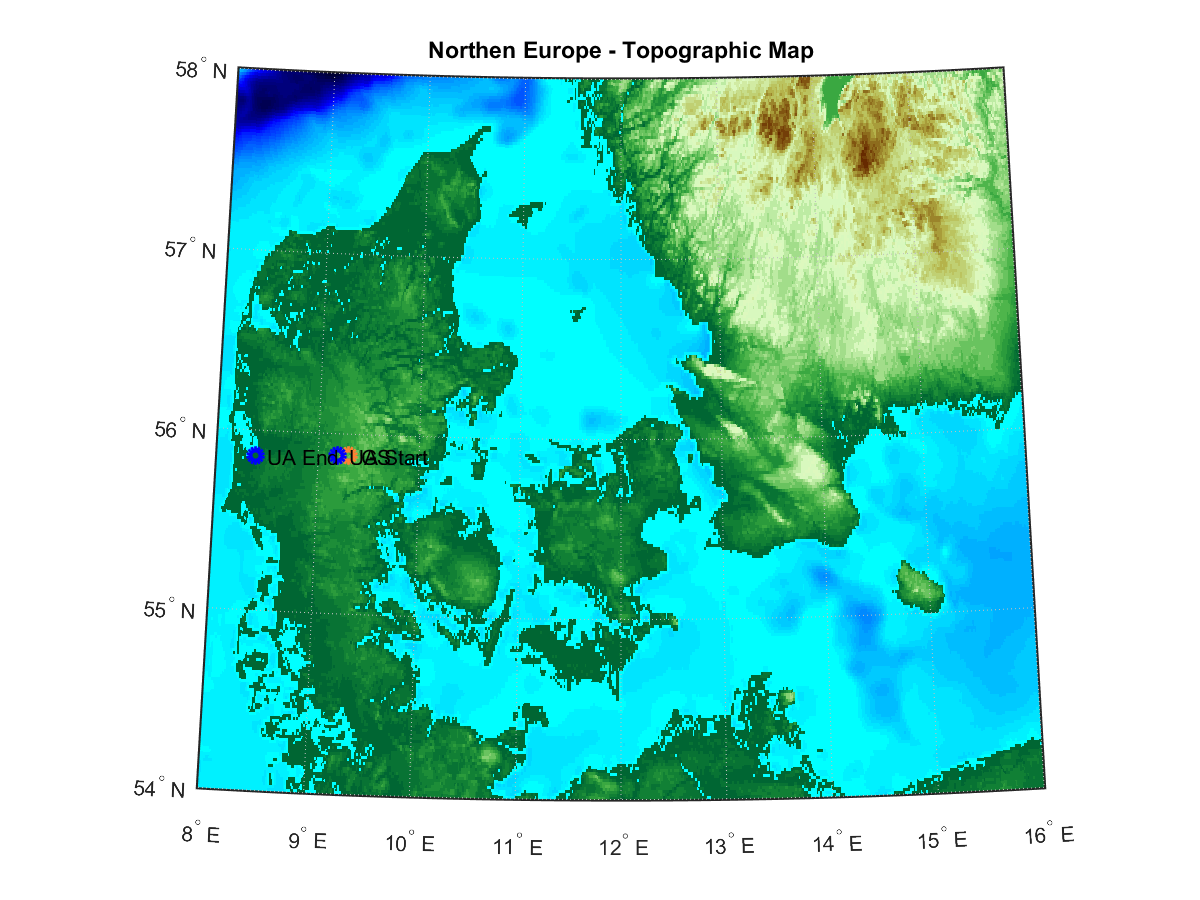
\includegraphics[scale=0.34]{figures/s2_map.png}}
	\hfill
	\subfigure[LOS and Distance]{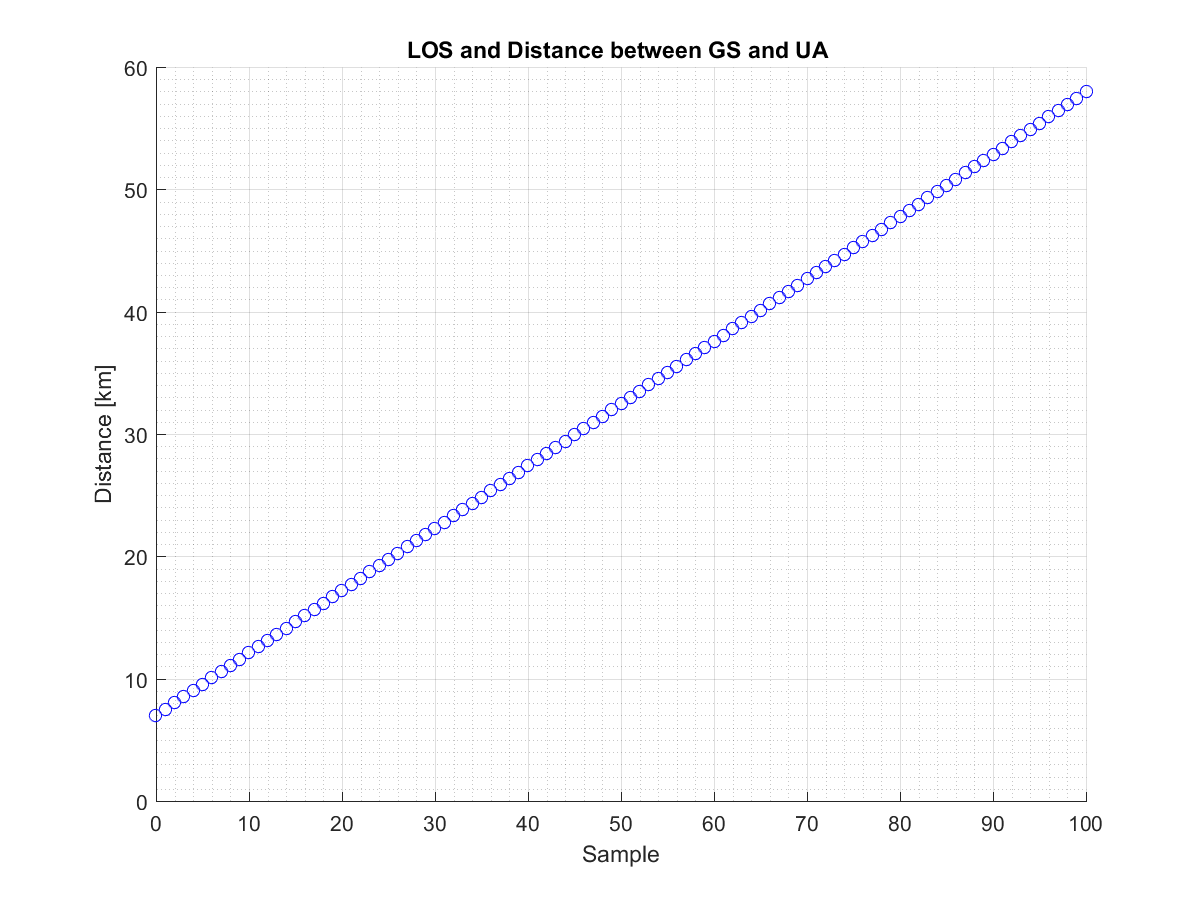
\includegraphics[scale=0.34]{figures/s2_los.png}}
	\hfill
	\caption{Mountain Scenario}
	\label{fig:s2_map}
\end{figure}


\subsection{Ground Station}
In this scenario, the UA is on the left side of the GS as is illustrated on Figure \ref{fig:s2_map}. As was explained in scenario 1, due to the chosen body frame coordinate of the GS, the optimal azimuth angle is always negative. On the other hand, the UA is flying away from the GS in a straight line which results in an almost constant azimuth angle. 

The optimal elevation angle has a slightly decrease (bigger than in the previous scenario) during the whole movement. It starts with a higher value because the UA is close to the GS. While the UA is progressing towards the end point, the distance between both devices grows which causes a decrease in the antenna's $\phi_{OPTIMAL}$ angle. However, in this situation, the $\phi_{OPTIMAL}$ becomes negative on the 70th sample, which means that, in the point of view of the GS, it has a bigger altitude compared to the UA one. The $\phi_{OPTIMAL}$ can achieve negative values because the curvature of the Earth was taken into account.

\begin{figure}[H]
	\centering
	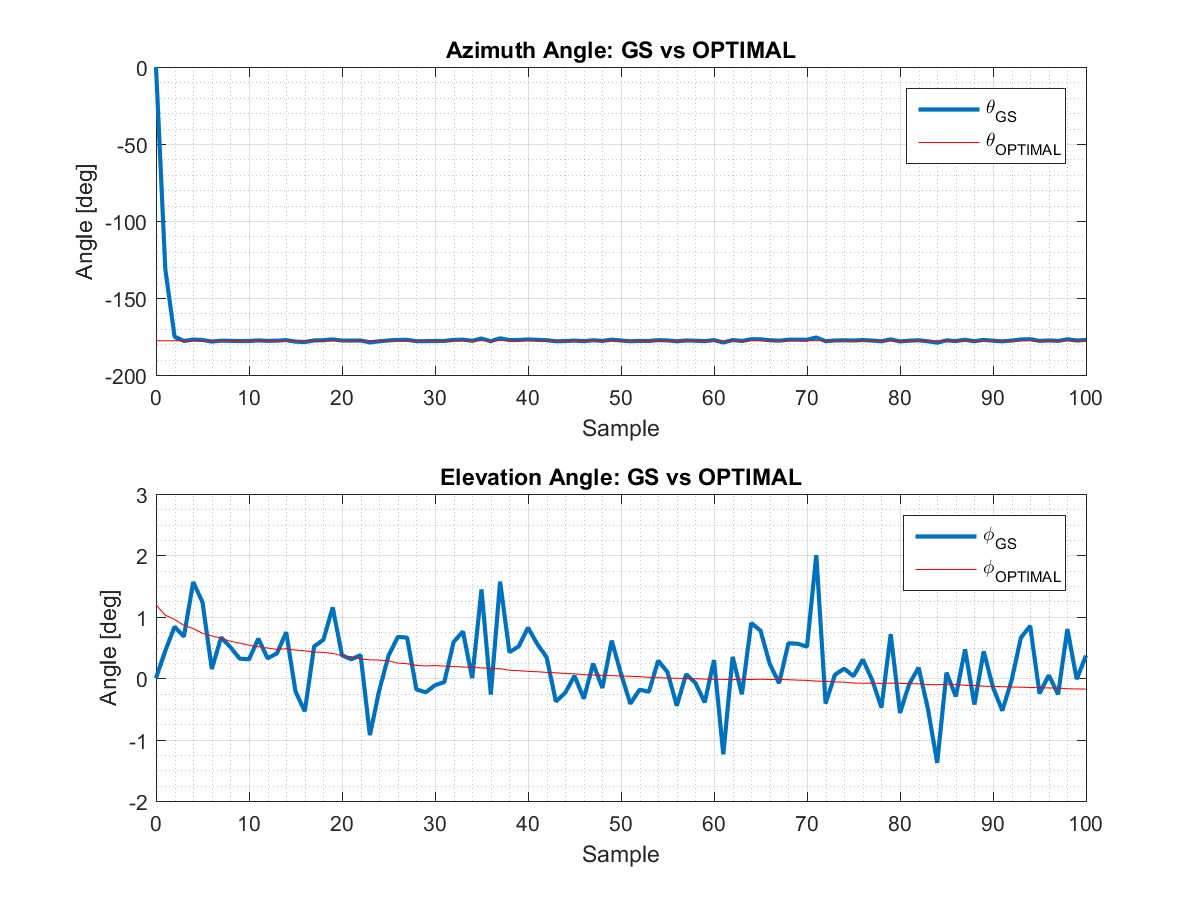
\includegraphics[scale=0.75]{figures/s2_gs.png}
	\caption{Azimuth and elevation angles of GS following the optimal angle}
	\label{fig:s2_gs}
\end{figure}

\subsection{Unmanned Aircraft}
The optimal and the real Azimuth angle in Figure \ref{fig:s2_ua} have the same behaviour, despite of the different values that the lines show. This means that due to the different conventions applied in each variable (section \ref{sec:scenario1}), the lines are not overlapped but they represent the same angle.

As was explained before, the UA is flying away from the GS which also implies that the reference of the body frame is pointing to the end point. Therefore, it demands that the antenna of the UA is pointing back in order to keep the connection with the GS. 

The elevation angle has a similar behaviour of the one of the GS. However, in this case, the antenna of the UA is pointing down because the altitude of the UA is bigger than the GS one. During the flight the angle of the antenna is increasing.


\begin{figure}[H]
	\centering
	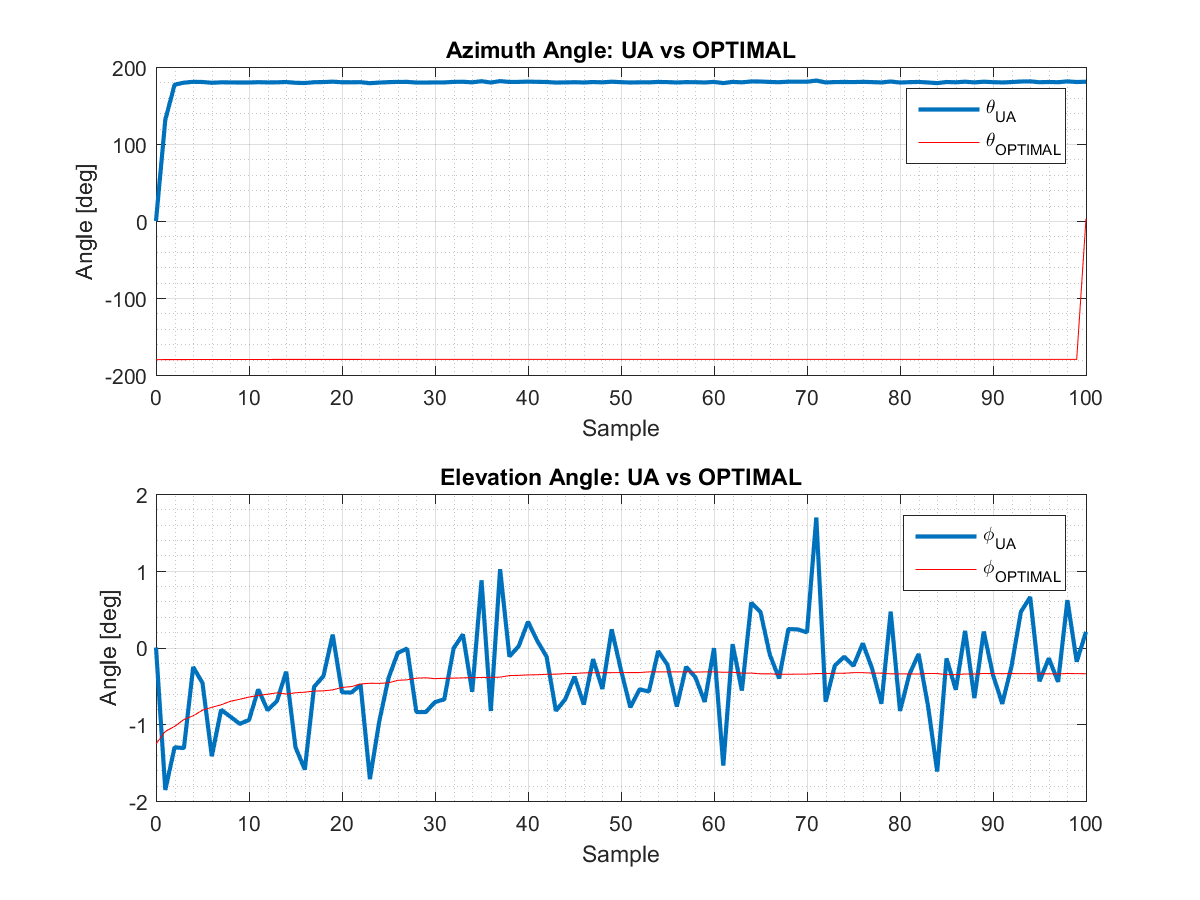
\includegraphics[scale=0.75]{figures/s2_ua.png}
	\caption{Azimuth and elevation angles of UA following the optimal angle}
	\label{fig:s2_ua}
\end{figure}


\subsection{Power}
In Figure \ref{fig:s2_power} the power at the receiver antenna of the GS antenna can be seen. In the beginning the power in the receiver is small (-100dBm) because the antennas are not pointing at each other. Although, after 4 samples, the connection is accomplished and the power reaches its maximum. 

During the flight the path losses are increasing since the UA is flying away from the GS. This causes a decrease in the power of the receiver.

\begin{figure}[H]
	\centering
	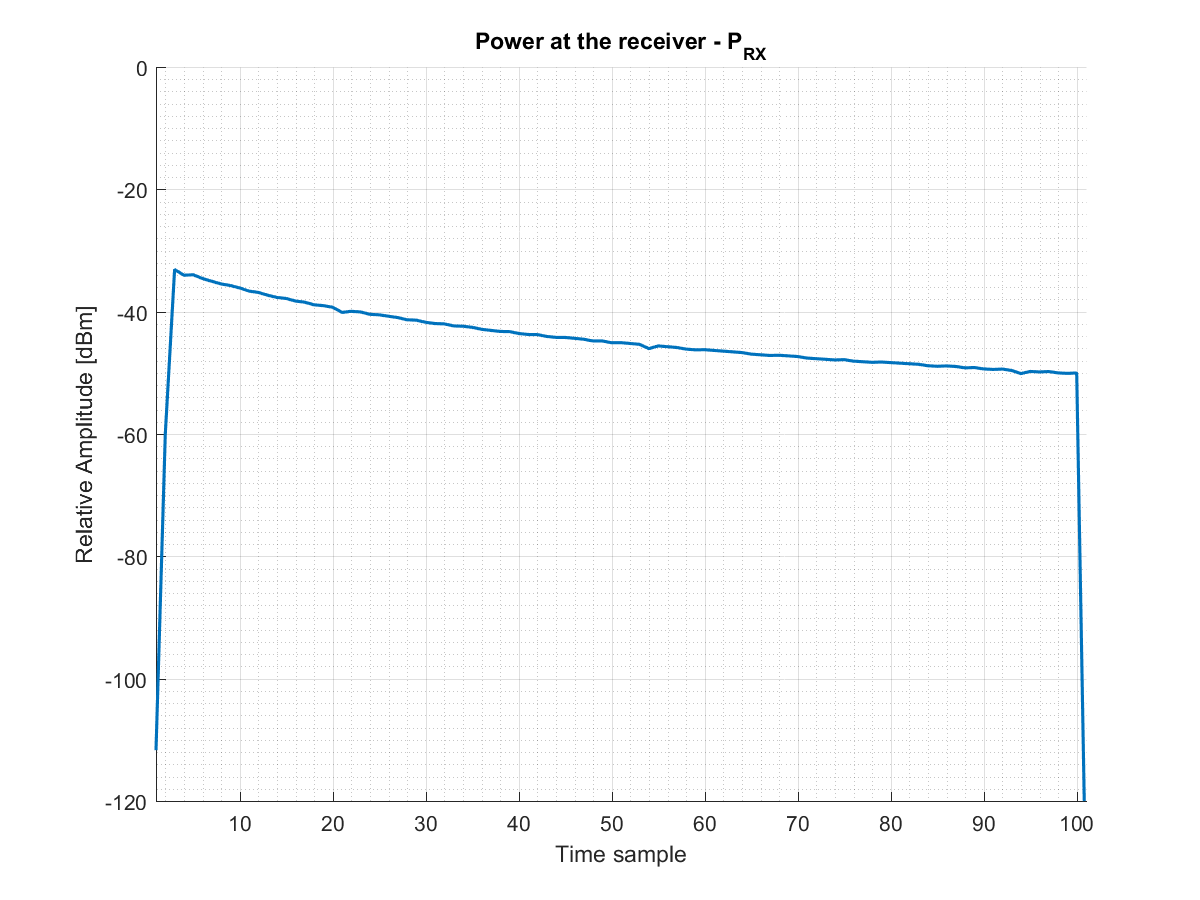
\includegraphics[scale=0.75]{figures/s2_power.png}
	\caption{Power at the receiver's antenna (GS)}
	\label{fig:s2_power}
\end{figure}

